\chapter{Analyse}

In diesem Kapitel wurden die betrachteten Veranstaltungen zunächst eingegrenzt.
Anschließend wurde eine Organisationsanalyse durchgeführt, um die verschiedenen
Phasen einer Veranstaltung einzubeziehen. Die Phasen „Umsetzung“, „Durchführung“
und „Schließung“ wurden hierbei näher analysiert. Basierend auf den Ergebnissen
der Organisationsanalyse wurden eine Benutzer- und Kontextanalyse durchgeführt.
Die Zielgruppen des Frameworks wurden festgelegt und für die Konzeption
relevante Besonderheiten herausgearbeitet. In einer abschließenden
Kontextanalyse wurden die verschiedenen Kontexte der Nutzung des Frameworks
aufgezeigt und auf die mit ihnen einhergehenden Herausforderungen eingegangen.


\section{Datenquellen}

Im Rahmen der Analyse wurden verschiedene Datenquellen genutzt. Eine
wissenschaftliche Literaturrecherche wurde zwischen dem 26.07.2021 und
11.08.2021 durchgeführt. Verschiedene vergleichbare Projekte wurden im Rahmen
einer Internetrecherche ermittelt. Die Ausarbeitung und Evaluation der
EMI-Award-App wurde als Quelle genutzt. Zudem wurden Interviews mit
Veranstaltenden und Teilnehmenden durchgeführt. Die Interviews fanden zwischen
dem 5.09.2021 und 17.09.2021 statt. \\
Zur Literaturrecherche wurden die digitalen Bibliotheken ACM Digital Library
(\url{https://dl.acm.org/}) und Google Scholar
(\url{https://scholar.google.de/}) genutzt. Es wurden Begriffe aus den Bereichen
Event Management (\emph{Event Management, Event Evaluation, Event Experience,
    Event Tracking}) und UX (\emph{Attention Economy, Attention Management,
    Information Overload, Digital Burnout, Overchoice, Web Animation, Animation UX,
    UX Micro Interaction, Animation Usability}) zur Suche verwendet. \\
Die Interviews mit Veranstaltenden und Teilnehmenden wurden qualitativ und
semistrukturiert, mit Hilfe eines dafür entworfenen Interviewleitfadens (siehe
Anhang A), durchgeführt. Bei den Veranstaltenden handelt es sich um Personen mit
praktischer Erfahrung in der Organisation von Veranstaltungen. In Tabelle
\ref{table:ver-soz} und Tabelle \ref{table:teil-soz} sind Details zu den
befragten Personen aufgelistet. Die IDs der interviewten Personen werden im
Verlauf der Analyse referenziert.

\begin{table}[htpb]
    \def\arraystretch{1.25}
    \centering
    \caption{Soziodemografische Daten der Veranstaltenden}
    \label{table:ver-soz}
    \begin{tabular}{lcll}
        \uzlhline
        \uzlemph{ID} & \uzlemph{Geschlecht} & \uzlemph{Alter} &
        \uzlemph{Vorerfahrung}                                                \\
        \uzlhline V1 & w                    & 40 - 59 J.      & Verschiedene
        Veranstaltungen, verteilt über 11 Jahre                               \\
        V2           & m                    & 18 - 25 J.      & Mehrere große
        Veranstaltung (>2000 Teilnehmende)                                    \\
        \uzlhline
    \end{tabular}
\end{table}

\begin{table}[htpb]
    \def\arraystretch{1.25}
    \centering
    \caption{Soziodemografische Daten der Teilnehmenden}
    \label{table:teil-soz}
    \begin{tabular}{lclcl}
        \uzlhline
        \uzlemph{ID}                     & \uzlemph{Geschlecht} & \uzlemph{Alter} &
        \uzlemph{EMI-Award-App genutzt?} & \uzlemph{Tätigkeit}                        \\
        \uzlhline T1                     & w                    & 18 - 25 J.      & j
                                         & Student:in                                 \\
        T2                               & m                    & 18 - 25 J.      & j
                                         & Student:in                                 \\
        T3                               & w                    & 18 - 25 J.      & j
                                         & Student:in                                 \\
        T4                               & m                    & 18 - 25 J.      & n
                                         & Student:in                                 \\
        T5                               & w                    & 40 - 59 J.      & n
                                         & Berufstätig                                \\
        \uzlhline
    \end{tabular}
\end{table}


\section{Definition: Veranstaltung} \label{sec:analysis-def}

Bevor die verschiedenen Aufgaben, Probleme und Benutzergruppen analysiert werden
können, müssen Umfang und Typ der Veranstaltung festgelegt werden. In der
Literatur sind viele verschiedene Definitionen zum Begriff „Veranstaltungen“ zu
finden, welche sich in Umfang und Inhalt stark unterscheiden. Dies ist der
Flexibilität der räumlichen und zeitlichen Dimension von Veranstaltungen, sowie
Teilnehmeranzahl und Sektor geschuldet. \textcite{Getz2007} definiert
Veranstaltungen beispielsweise als zeitliche Phänomene. Bei geplanten
Veranstaltungen wird das Veranstaltungsprogramm oder der Zeitplan im Allgemeinen
detailliert geplant und im Voraus gut bekannt gemacht. Geplante Veranstaltungen
sind in der Regel auch auf bestimmte Orte beschränkt, wobei es sich um eine
bestimmte Einrichtung, eine sehr große Freifläche oder viele Orte handeln kann.
\textcite{Bladen2017} definieren Veranstaltungen als zeitlich begrenzte und
zweckgebundene Zusammenkünfte von Menschen definiert.

Im Rahmen dieser Arbeit werden Veranstaltungen betrachtet, welche in ihrer
zeitlichen Dimension uneingeschränkt sind, jedoch räumlich verteilt angesetzt
sind. Konkret können die betrachteten Veranstaltungen wenige Stunden, Wochen
oder ohne festgelegtes Ende stattfinden. Zudem verteilen sich die Aktivitäten
der Veranstaltung, sodass ein signifikanter Abstand zwischen ihnen vorliegt.
Dies kann mindestens die Aufteilung auf verschiedene Räumlichkeiten sein, bis
hin zur Verteilung über verschiedene Stadtteile.


\section{Organisationsanalyse} \label{sec:analysis-org}

% Masterarbeit_Holtz  Aufgabenanalyse!!!
Die hier analysierte Vorgehensweise in der Organisation von Veranstaltungen
basiert auf dem EMBOK-Model \cite{Silvers2013} und den Aussagen der interviewten
Veranstaltenden. Typischerweise lässt sich die Organisation von Veranstaltungen
in 5 Phasen (s. \autoref{fig:embok-phases}) gliedern: Initiation, Planung,
Umsetzung, Durchführung und Schließung. Die Vorgehensweise in den Phasen
gestaltet sich wie folgt:

\begin{enumerate}
    \setlength{\itemsep}{1em}
    \item \textbf{Initiation} \\
          Es wird geforscht, um ein Konzept zu erstellen und zu validieren.
          Umfang und Kontext sowie Ziele und Aufgaben werden festgesetzt.
    \item \textbf{Planung} \\
          Anforderungen und Spezifikationen werden festgehalten. Hierzu zählen
          die stattfindenden Aktivitäten, sowie die Art der Organisation und
          erforderliche Ressourcen.
    \item \textbf{Umsetzung} \\
          Alle Waren und Dienstleistungen werden in Auftrag gegeben und
          koordiniert. Der Fokus liegt unter anderem auf der Überwachung und
          Überprüfung des Umfangs und Zeitplans, sowie der Kosten und Qualität.
    \item \textbf{Durchführung} \\
          Die veranstaltungsbezogenen Aktivitäten werden aufgenommen. Ab Beginn
          dieser Phase ist der Handlungsrahmen stark eingeschränkt, wodurch der
          Fokus auf der Überwachung der Veranstaltung liegt.
    \item \textbf{Schließung} \\
          Nach Abschluss der Veranstaltung werden Daten gesammelt, ausgewertet
          und weitergegeben. Das Ziel ist die Dokumentation der Erkenntnisse für
          weitere Veranstaltungen.
\end{enumerate}

\begin{figure}[htpb]
    \centering
    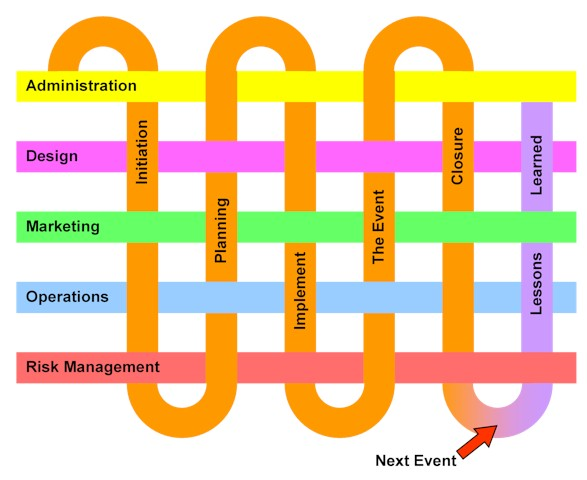
\includegraphics[width=\textwidth]{embok_phases.jpg}
    \caption{Die Phasen der Veranstaltungsorganisation \cite{Silvers2013b}. Die
        verschiedenen Phasen (vertikal) bilden die Grundlage einer
        Veranstaltung. Verwoben sind diese mit Wissensdomänen (horizontal).
        Sollte einer der Fäden verschwinden, wird das gesamte Geflecht
        geschwächt.}
    \label{fig:embok-phases}
\end{figure}

Da das Ziel dieser Arbeit die Unterstützung ab der Umsetzung ist (s.
\autoref{sec:goals}), werden die Phasen „Umsetzung“, „Durchführung“ und
„Schließung“ näher betrachtet.

\subsection{Umsetzung} \label{sec:analysis-org-umsetzung}

In dieser Phase werden die herausgearbeiteten Pläne umgesetzt. Hierbei werden
Umfang, Zeitpläne, Kosten, Kommunikation und Risiken überwacht und kontrolliert,
um die plangemäße Ausführung sicherzustellen. Weitere Arbeits-/Hilfskräfte
werden engagiert, um bei der Umsetzung mitzuwirken. Für den Erfolg der
Veranstaltung ist die effektive Kommunikation wichtig. Um diese zu
gewährleisten, muss eine Kommunikationsinfrastruktur für Organisierende,
Mitwirkende und externe Dienstleister eingeführt werden. Hilfskräfte müssen in
die Kommunikationsinfrastruktur eingewiesen werden. Aufgrund von mangelnden
technischen Fähigkeiten können bei komplexeren Infrastrukturen Probleme
auftreten (V2).

\subsection{Durchführung} \label{sec:analysis-org-durchfuehrung}

Mit Beginn der Durchführung ändert sich die Dynamik der Veranstaltung bedeutend.
Aufgrund der Anwesenheit von Teilnehmenden sind tiefgreifende Änderungen nun
nicht mehr möglich und beschränken sich auf die Behebung von kleinen Problemen
(V2). Hingegen wird die wichtigste Aufgabe die Überwachung der Veranstaltung.
Unter besonderer Beobachtung stehen logistische Tätigkeiten, sowie unerwartet
auftretende Probleme (V1, V2). Diese können u. a. durch Teilnehmende,
stattfindende Aktivitäten oder die Umgebung der Veranstaltung ausgelöst werden.
\\
Während Probleme, welche die Durchführung der Veranstaltung direkt
beeinträchtigen könnten, streng beobachtet und behoben werden, stehen die
Interaktionen und Erfahrungen der Teilnehmenden zunächst im Hintergrund.
Abgesehen von kritischem Feedback, wird die Erfahrung erst während der
Schließung erfasst und ausgewertet (V2).

\subsection{Schließung} \label{sec:analysis-org-schliessung}

% Bedeutung Evaluation aus Finischen Case S.57-59 Mischung Quantitativ &
% Qualitativ Evaluation S.61

Zur Schließung der Veranstaltung wird die Evaluation zur bedeutendsten Aufgabe.
Feedback und Daten werden von organisierender Seite gesammelt. Hierbei wird
zwischen \textit{weichen} und \textit{harten Daten} unterschieden. Harte Daten
bestehen aus Teilnehmerzahlen, Andrang an verschiedenen Aktivitäten, Dauer,
Einkommen und weiteren zählbaren Merkmalen. Im Vergleich dazu bestehen weiche
Daten u. a. aus Beschwerden, Konflikten, Problemen, Komplimenten, Reaktionen und
Empfehlungen. Mitwirkende, Hilfskräfte und die Organisierenden werden meist dazu
in einer Nachbesprechung befragt (V1,V2). Das Feedback von Teilnehmenden wird
oft nur passiv vor Ort vom Personal erfasst und weitergegeben oder beschränkt
sich auf Familie und Freunde (V2). Die erfassten Erkenntnisse werden
dokumentiert, um auf das Wissen in der nächsten Veranstaltung zurückgreifen zu
können.


\section{Benutzeranalyse} \label{sec:analysis-user}

Um die Funktionen des Frameworks zielgruppengerecht gestalten zu können, werden
in diesem Abschnitt die Benutzergruppen des Frameworks festgelegt und näher
analysiert. Zu den Benutzergruppen gehören Veranstaltende, sowie Teilnehmende
einer Veranstaltung.

\subsection{Veranstaltende}

% !===Veranstaltende===!

% Phasen der Veranstaltung
%   - Wo wird für Veranstalter angesetzt?
%   - Wie werden die Prozesse unterstützt?
%   - Was ist der Mehrwert?

% Herkömmliche Planung nur im Voraus
%   - Durch App mehr ad hoc handeln
%       - Push
%       - Feedback
%       - Reaktionen

% Wann setzt die App an?
%   - Werbephase?
%       - "Innovations"-Boost?
%   - Durchführung (duh)

Inzwischen existieren weltweit tausende Einrichtungen, welche formale
Qualifikationen und Ausbildungen im Veranstaltungsmanagement anbieten. Jedoch
sind diese Qualifikationen nicht einheitlich festgelegt, was zu
unterschiedlichen Schwerpunkten, Umfang, Vermittlungsart und letztendlich
erworbenen Qualifikationen führt \cite{Bladen2017}. In Deutschland gibt es den
anerkannten Ausbildungsberuf des/der Veranstaltungs\-kaufmann/-frau. Die
Aufgaben sind hierbei die Konzipierung und Organisation des kaufmännischen
Aspektes von Veranstaltungen \cite{Kultusministerkonferenz2001}. Die Aufgaben
eines/r Event Manager/in umfassen zusätzlich die allgemeine Organisation und
Aufgaben im Marketing \cite{BundesagenturfurArbeit2021}. Jedoch ist die
Berufsbezeichnung „Event Manager/in“ rechtlich nicht geschützt. \\
Zudem bedarf es in Deutschland keiner formalen Qualifikation, um eine
Veranstaltung beliebiger Größe zu organisieren. Dementsprechend können keine
bestimmten Qualifikationen für Veranstaltende angenommen werden.

\subsection{Teilnehmende}

Die Teilnehmenden einer Veranstaltung unterscheiden sich stark in ihren
soziodemografischen Daten je nach Typ der Veranstaltung. Im Kontext der Arbeit
sind besonders Alter, Technikaffinität und körperliche, seelische, geistige oder
Sinnesbeeinträchtigungen. Für die Betrachtung in dieser Arbeit wird das Alter
der Teilnehmenden auf 16 - 60 J. begrenzt. Zudem wird die sichere grundlegende
Umgangsweise mit einem Smartphone vorausgesetzt.

Da die Literatur zu Event Management ihren Fokus auf die Organisation legt, sind
nur wenig Informationen zur Sicht der Teilnehmenden und ihren Hürden vorhanden.
Als Messwerte für eine erfolgreiche Veranstaltung werden meist
geschäftsrelevante Werte wie z. B. verkaufte Tickets, Teilnehmerzahlen, Umsatz
oder öffentliche Aufmerksamkeit verwendet, welche wenig über die Erfahrung der
Teilnehmenden aussagen. In Interviews wurden die Teilnehmenden gebeten zu
begründen, was eine gewählte Veranstaltung zu ihrem persönlichen Favoriten macht
(s. \autoref{table:teil-fav}).

\begin{table}[htpb]
    \def\arraystretch{1.25}
    \centering
    \caption{Merkmale von positiv empfundenen Veranstaltungen}
    \label{table:teil-fav}
    \begin{tabular}{ll}
        \uzlhline
        \uzlemph{Grund}               & \uzlemph{ID} \\
        \uzlhline  Sozialer Austausch & T1, T2       \\
        Innovative Technik            & T2           \\
        Persönliche Bindung           & T4           \\
        Gute Musik                    & T3           \\
        Einfache Wegfindung           & T5           \\
        Neues Wissen                  & T5           \\
        \uzlhline
    \end{tabular}
\end{table}

% Interviews anhören nach Favoriten Antwort

% !===Teilnehmende===!

% !Alter, Soziale Schicht, Technik Affinität

\section{Kontextanalyse} \label{sec:analysis-context}

In diesem Abschnitt werden der zeitliche und räumliche Kontext untersucht. Aus
der Beschreibung in \autoref{sec:goals} geht der Fokus auf die Unterstützung von
Veranstaltenden und Teilnehmenden hervor. Die Unterteilung der Benutzergruppen,
wie in \autoref{sec:analysis-user} beschrieben, ist zu beachten. Hieraus ergeben
sich unterschiedliche räumliche und zeitliche Kontexte für Veranstaltende und
Teilnehmende.

Die Unterstützung der Veranstaltenden findet in verschiedene Phasen der
Organisation statt. Der zeitliche Kontext kann mit Blick auf
\autoref{sec:analysis-org} in vor, während und nach einer Veranstaltung
unterteilt werden. Vor der Durchführung einer Veranstaltung ist insbesondere die
Vorbereitung von Aktivitäten und Absicherung von Dienstleistungen oder Waren
wichtig. Während der Veranstaltung hingegen findet ein starker Fokuswechsel auf
die Beobachtung und schnelle Behebung von Problemen statt. Nach einer
Veranstaltung sind die Datensammlung und Auswertung, sowie der Wissenstransfer
von Bedeutung. \\
Auch beschränken sich die betrachteten Veranstaltungen während der Durchführung
auf den in \autoref{sec:analysis-def} beschriebenen örtlichen Bereich, woraus
sich ein weites gehend unbeschränkter räumlicher Kontext ergibt. Vor und nach
der Veranstaltung werden komplexe Informationen eingetragen oder ausgewertet. Da
die Bildschirmgröße einen großen Einfluss auf die effiziente Verarbeitung von
Informationen hat, wird hierfür von einem Arbeitsplatz mit großem Bildschirm
ausgegangen. Somit ergibt sich ein räumlich eingeschränkter Kontext vor und nach
der Veranstaltung. Folglich wird während der Veranstaltung ein mobiles System
zur Überwachung benötigt, wobei die Bedingungen vor und nach der Veranstaltung
ein stationäres System befürworten.

Für Teilnehmende ist der Kontext ebenfalls in vor, während und nach der
Veranstaltung aufgeteilt. Der zeitliche Kontext während der Veranstaltung ist
hierbei am bedeutendsten. Auch für Teilnehmende gilt der in
\autoref{sec:analysis-def} beschriebene örtliche Bereich, woraus sich ebenfalls
ein unbeschränkter räumlicher Kontext ergibt. Folglich muss das System für die
Teilnehmenden mobil einsetzbar sein.

% Der Framework muss für Teilnehmende folglich mobil einsetzbar sein.

% Trennung Kontext Veranstalter - Teilnehmer
% - Zusammentreffen erst ab Durchführung
% - Unterschiede im Kontext

% Achsen der Zugänglichkeit
%   - Körperliche Einschränkungen
%       - Blindheit
%       - Motorische Einschränkungen
%   - technische Barriere
%       - Geräte (iOS/Android)
%       - Affinität, besonders ältere Generationen
%       - Leistung der Geräte


\section{Ähnliche Projekte}

An dieser Stelle werden drei ähnliche Anwendungen betrachtet. Es existiert
bereits eine beträchtliche Anzahl von Plattformen und Anwendungen für die
digitale Unterstützung von Veranstaltungen. Der Fokus dieser Plattformen liegt
jedoch häufig auf Konferenzen, welches an der \textit{Attendify} Plattform
gezeigt wird. Im Gegensatz hierzu stehen die \textit{Mobile Event App} und
\textit{EMI-Award-App}, welche Funktionen für hybride oder nur örtlich
stattfindende Veranstaltungen bieten.

\subsection{EMI-Award-App}

% Tech-Stack
%   - Hat sich größten teils bewährt
%   - Web-App mit PWA Funktionalität

% Mockups
%   - Bereits getestet
%   - Grobe Struktur beibehalten

Die \textit{EMI-Award-App} ermöglichte das augmentierte Besuchen, Einsehen und
Bewerten der EMI-Award-Projekte und bildet die Grundlage dieser Arbeit (s.
\autoref{sec:goals}). Speziell wurden dafür an verschiedenen Standorten Schilder
mit QR-Codes angebracht, welche mit einem QR-Code-Reader oder der App gescannt
werden konnten (s. \autoref{fig:emi-qr-code}).

\begin{figure}[htpb]
    \centering
    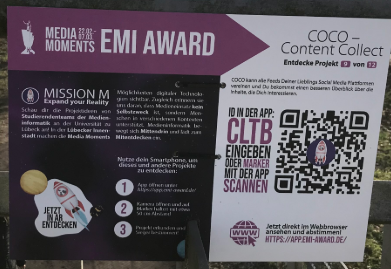
\includegraphics{emi_schild.png}
    \caption{Schild eines Projektstandortes mit QR-Code}
    \label{fig:emi-qr-code}
\end{figure}

Beim ersten Aufruf der App wird dem Nutzenden eine kleine Einführung in die App
und ihren Hintergrund gegeben. Dies geschieht über eine interaktive Slideshow.
Nach dem Bestätigen der letzten Slide werden Nutzende zur interaktiven Karte
geführt (s. \autoref{fig:emi-intro-map}). Auf dieser werden die Projektstandorte
durch verschiedenfarbige Icons von Planeten (\textgraphics{emi_planet.png})
dargestellt. Durch das Antippen eines Standorts wurde eine Kurzinformation zum
jeweiligen Projekt angezeigt. Außerdem wurde der Standort des Nutzenden
angezeigt, insofern die Berechtigungen dazu gegeben wurden.

\begin{figure}[htpb]
    \begin{minipage}{.5\textwidth}
        \centering
        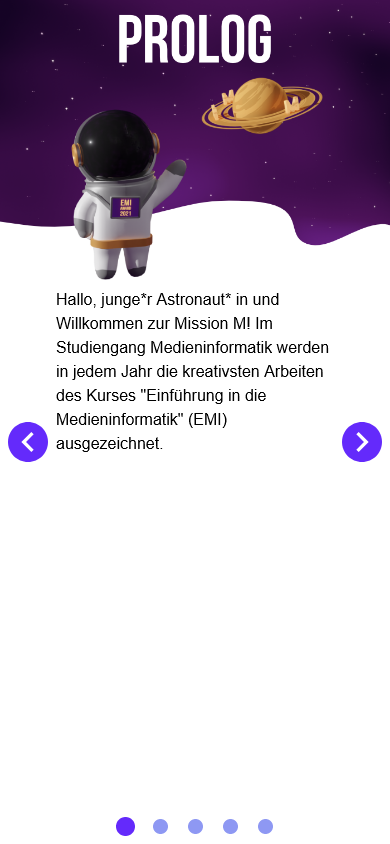
\includegraphics[width=.6\linewidth]{emi_prolog.png}
    \end{minipage}%
    \begin{minipage}{.5\textwidth}
        \centering
        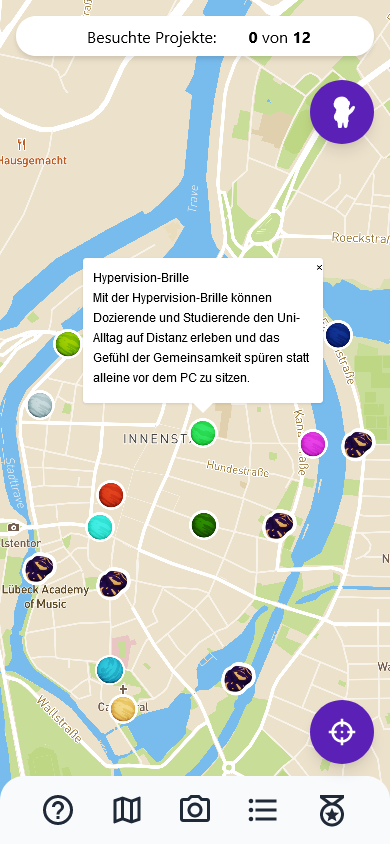
\includegraphics[width=.6\linewidth]{emi_map.png}
    \end{minipage}
    \caption{Einführung und interaktive Karte mit Projektstandorten}
    \label{fig:emi-intro-map}
\end{figure}

Um die vollständigen Informationen eines Projekts einzusehen, musste der
Standort erst virtuell besucht werden. Dies geschah über das Scannen des
QR-Codes auf dem Schild des Standorts (s. \autoref{fig:emi-qr-code}) oder der
manuellen Eingabe eines spezifischen Codes. Nach erfolgreichem Scannen oder
Eingeben des Codes wurde eine virtuelle Szene angezeigt. In dieser musste ein
Planet angetippt werden, um den Vorgang abzuschließen (s. \autoref{fig:emi-ar}).
Je nach benutztem Gerät wurde die Szene per Augmented Reality (AR) oder Virtual
Reality angezeigt (VR). Zudem wurde die Anzahl der besuchten Standorte in der
Karten- und Projektansicht anhand eines Fortschrittsbalkens angezeigt. Die
vollständigen Informationen der Projekte enthielten mediale Inhalte, eine
detaillierte Beschreibung und die Autoren des Projekts. Zusätzlich konnte das
Projekt mit einer vorgegebenen Auswahl bewertet werden (s.
\autoref{fig:emi-project}).

\begin{figure}[htpb]
    \begin{minipage}{.5\textwidth}
        \centering
        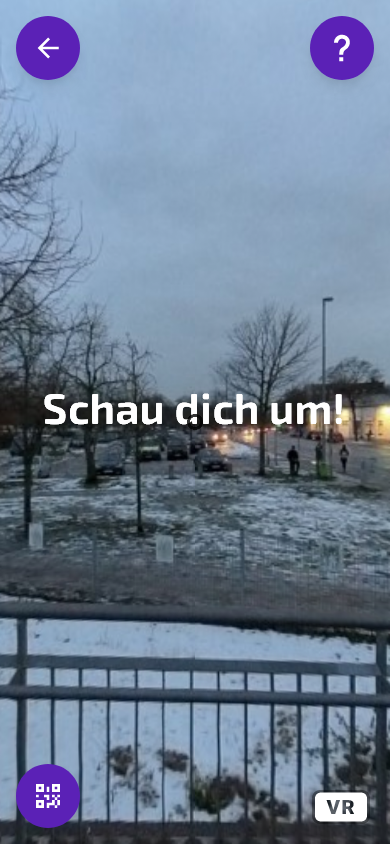
\includegraphics[width=.6\linewidth]{emi_ar-1.png}
    \end{minipage}%
    \begin{minipage}{.5\textwidth}
        \centering
        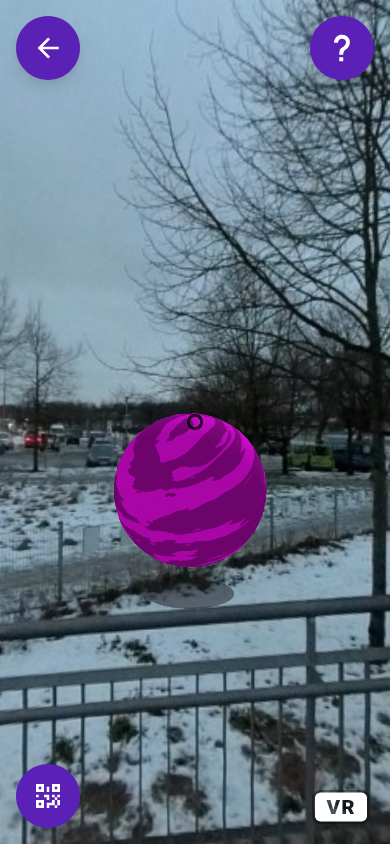
\includegraphics[width=.6\linewidth]{emi_ar-2.png}
    \end{minipage}
    \caption{AR/VR Szene während des virtuellen Besuchs}
    \label{fig:emi-ar}
\end{figure}

\begin{figure}[htpb]
    \begin{minipage}{.5\textwidth}
        \centering
        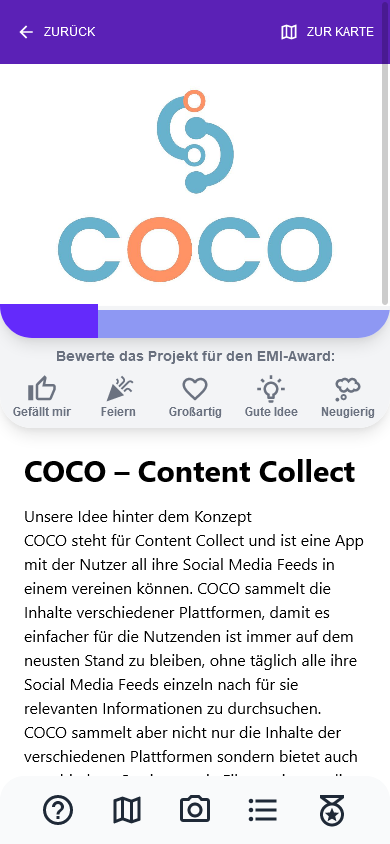
\includegraphics[width=.6\linewidth]{emi_project-1.png}
    \end{minipage}%
    \begin{minipage}{.5\textwidth}
        \centering
        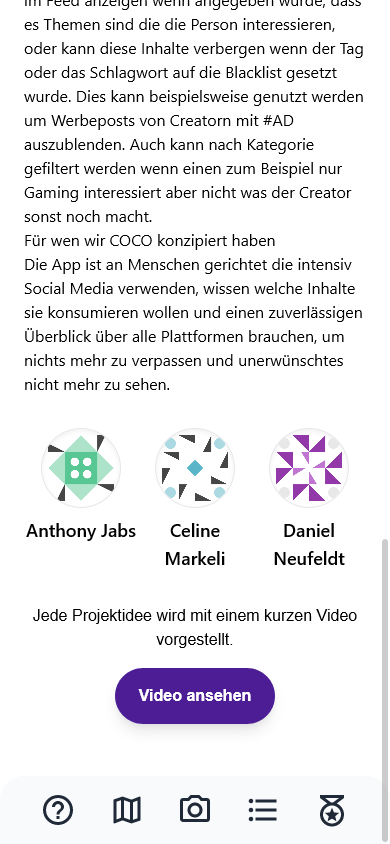
\includegraphics[width=.6\linewidth]{emi_project-2.png}
    \end{minipage}
    \caption{Einzelansicht eines Projekts}
    \label{fig:emi-project}
\end{figure}

Des Weiteren konnten verschiedene Abzeichen für bestimmte Aktionen erhalten
werden. Aktionen waren z. B. das Besuchen einer bestimmten Anzahl von Projekten
oder Benutzen von bestimmten Funktionen. Alle Abzeichen und ihr Fortschritt
konnten in einer Übersicht eingesehen werden (s. \autoref{fig:emi-achievments}).
Bestimmte Abzeichen wurden in mehreren Stufen freigeschaltet oder blieben bis
zum Erhalt verborgen. \\
Zudem wurden die gesammelten „Awardteile“ angezeigt. Awardteile sind sammelbare
Objekte, welche auf der Karte mit einem Meteorit-Symbol
(\textgraphics{emi_meteorit.png}) gekennzeichnet waren. Beim Annähern an die
gezeigten Standorte wurde eine Schaltfläche hervorgehoben, welche durch Antippen
das entsprechende Awardteil sammelt.

\begin{figure}[htpb]
    \centering
    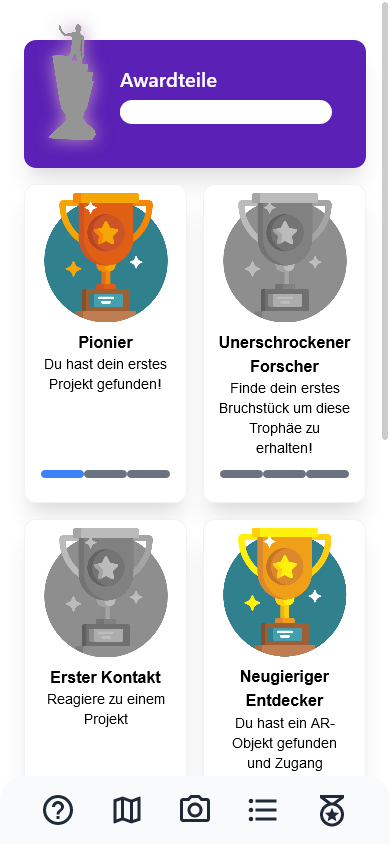
\includegraphics[width=.3\textwidth]{emi_achievements.png}
    \caption{Abzeichen- und Awardteilansicht}
    \label{fig:emi-achievments}
\end{figure}

Außerdem werden die genannten Funktionen in der App durch eine Slideshow
erklärt, welche jederzeit über die Navigationsleiste erreichbar ist (s.
\autoref{fig:emi-help}).

\begin{figure}[htpb]
    \centering
    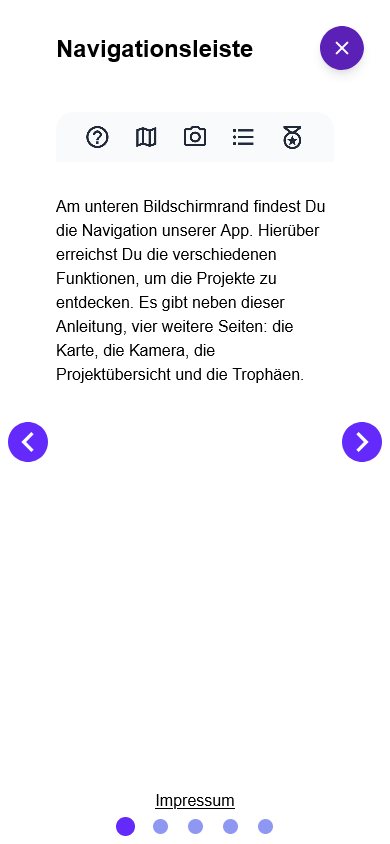
\includegraphics[width=.3\textwidth]{emi_help.png}
    \caption{Eine Seite der In-App-Anleitung}
    \label{fig:emi-help}
\end{figure}

Die EMI-Award-App wurde als progressive Web-App (PWA) realisiert und war unter
\url{https://app.emi-award.de} verfügbar.

\subsection{Mobile Event App}



\subsection{Attendify}



\section{Problemanalyse} \label{sec:analysis-problems}

Während Planung, Durchführung und Nachbereitung von Veranstaltungen können
Probleme auftreten, welche die Organisation erschweren. Ähnlich treten bei der
Teilnahme Probleme auf, welche die Erfahrung beeinträchtigen können.

\subsection{Organisation}

In der Organisation von Veranstaltungen treten vor allem Probleme in der
Kommunikation auf. Je nach Größe der Veranstaltung können eine Vielzahl an
Menschen an der Organisation beteiligt sein. Meist sind verschiedene digitale
Tools oder Plattformen zur Kommunikation erforderlich, um sich mit allen
Veranstaltenden zu verständigen (V2). Hier kann es zu Herausforderungen kommen,
auch Menschen mit geringem Technikverständnis einzuweisen (V2). Aber auch der
Kontakt zu Teilnehmenden spielt eine große Rolle. Jedoch ist der Kontakt während
einer Veranstaltung nur gering (V1, V2). Nach einer Veranstaltung fällt der
Kontakt ebenfalls sehr schwer (V1) oder wird komplett ausgelassen (V2).

Außerdem treten Probleme in der Übersicht über die Veranstaltung auf. Gerade bei
räumlich größeren Veranstaltungen gibt es keine direkte Übersicht über die
Teilnehmenden (V1). Oft werden für die Datensammlung nur Schätzungen verwendet
(V2). Jedoch ist die Reichweite ein wichtiger Indikator für Veranstaltende (V1).
Allgemein besteht die Datensammlung in der Nachbesprechung aus Aussagen von
Veranstaltenden oder deren Angehörigen und Freunden (V2).

Weitere Probleme treten in der Beeinflussung von Veranstaltungen während ihrer
Durchführung auf. Es besteht der Bedarf kleine Änderungen noch einfacher
vornehmen zu können (V1). Zudem mangelt es bei räumlich verteilten
Veranstaltungen an Möglichkeiten ein Gruppengefühl zu erzeugen (V1).

% !Durchführung

% Wenig Kontakt zu Teilnehmenden während der Veranstaltung (V1, V2)
% - Aber differenziert nach Typ der Veranstaltung (Nicht wenn Speaker)
% - Besonders Kontakt nach der Veranstaltung sehr schwer (V1)
% - Kein Kontakt danach (V2)

% Übersicht über Veranstaltung schwer
% - Keine direkte Übersicht über Teilnehmer (V1)
% - oder nur grobe Schätzungen (V2)
% - Aber Reichweite wichtig zu wissen (V1)

% Bedarf während der Veranstaltung noch eingreifen zu können / kleine Änderungen
% tätigen zu können (V1)

% Bedarf für besser Kommunikation während der Veranstaltung (V2)
% - Nachricht an alle Mitwirkendenen (V2)

% Bedarf Gruppengefühl erzeugen zu können (V1)

% Bei verteilten Projekten:
% - Lage der Projekte nicht einfach / manche vernachlässigt (V1)

% Gedanken zur Zugänglichkeit teils nicht (V1)
% - Teils aber auch schon (V2)
% - Leichterer Zugang als zur EMI-Award-App

% !Nachbereitung

% Richtiger Abschluss schwer (V1)
% - Besonders das Einholen von Feedback (V1,V2)
% - Feedback nur von Freunden, Familie, passive Beobachtung (V2)

% Die Interviews der Veranstaltenden bestätigen, dass die Überwachung der
% Aktivitäten nur auf der Makroebene erfolgt, da Interaktionen auf Mikroebene
% schwer zu verfolgen sind. Je nach Veranstaltungstyp liegt der Fokus auf der
% Sicherheit und Logistik der Veranstaltung. Evaluationen werden meist nach
% Veranstaltungen durchgeführt, jedoch nicht während Veranstaltungen. In
% seltenen Fällen wurde eine Evaluation vor der Veranstaltung durchgeführt, um
% die Erwartungen der Teilnehmenden zu erfassen.

% Einen weiteren Schwerpunkt stellt effiziente Kommunikation dar, welche zur
% schnellen Behebung von Problemen benötigt wird. Alle Mitglieder des Teams
% sollten ihre Umgebung im Blick haben und problematische Beobachtung
% unverzüglich kommunizieren können. Aus den Interviews ergab sich, dass die
% Kommunikation innerhalb des veranstaltenden Teams, aber auch besonders zu
% Teilnehmenden eine Herausforderung darstellt.

% Des Weiteren werden Evaluationen nur nach Abschluss der Veranstaltung
% durchgeführt. Hierbei werden teilweise nur persönliche Erfahrungen der
% Organisierenden und Helfenden zusammengetragen und ausgewertet. Dies ist der
% mangelnden Datenerhebung während der Veranstaltung zuzurechnen.

\subsection{Teilnahme}

% - Nachfrage nach Event-Assistenten
% - Wegfindung / Übersicht
% - Alle gesellschaftlichen Schichten
% - Alle Altersklassen
% - Menschen mit körperlichen Einschränkungen

% !===EMI-App===!

% Vorhandene Evaluationen und Erarbeitung der EMI-Award-App
%   - Ausweitung der Nutzenden
%   - Nutungskontext Veränderungen

% Marker-Problem
%   - Ausgedruckt
%       - nicht mehr (ohne großen Aufwand) änderbar
%       - Vandalismus

% !===Interviews===!

% Veranstaltende
%   - Erfassung des organisatorischen Ablaufs
%   - Feststellen der vorhandenen Probleme
%   - Lösungsansätze erkunden
%   - Evaluationsgrundlage erfahren
%   - Kommunikation erfassen

% Teilnehmende
%   - Bisherige Erfahrungen mit digitaler Anreicherung
%       - Positives & Negatives
%       - Bzw. überhaupt
%   - Hilfreiche Unterstützung erarbeiten
%   - Priorität des sozialen Austauschs
%       - Verschiedene Arten von Veranstaltungen
%   - Bevorzugte Informationsvermittlung (multi-modal)


% !===Erarbeitete Anforderungen / Funktionalitäten===!

% Die Durchführung mit veranstaltenden Personen erfasste relevante
% Veranstaltungstypen, sowie wertvolle Funktionen aus organisatorischer Sicht.
% Hingegen erfassten die Interviews mit teilnehmenden Personen Erfahrungen mit
% digital unterstützen Veranstaltungen und hilfreiche vorhandene und gewünschte
% Funktionen.

% - Alle gesellschaftlichen Schichten
% - Alle Altersklassen
% - Menschen mit körperlichen Einschränkungen


\section{Implikation für Konzeption} \label{sec:analysis-implic}

% Während der Veranstaltung Fokus Überwachung und Sicherstellung der Aktivitäten
% -> Die Stationsdashboards mit Nachrichten, Informationen und Übersicht zur
% Überwachung

% Mobiler Einsatz -> Betriebssysteme für Handys
%   - iOS vs Android https://gs.statcounter.com/os-market-share/mobile/europe/
%   - PWA / Web-App

% Stabilität und Zuverlässigkeit *sehr* wichtig
%   - Ausfall kann gesamtes Event lahmlegen
%   - Bei hoher Teilnehmeranzahl hohe Last

% Warum inclusive Design
%   - Menschen aller gesellschaftlichen Schichten nehmen an Veranstaltungen teil
%   - Jedem sollte die Chance geboten werden teilzunehmen

% Gruppengefühl, Soziale Interaktion -> Gruppenfunktion, Reaktionen

% Bessere Kommunikation -> Stationsdashboard